\section{Clustering of tiles}
\label{sec:clusters}

As discussed in \secref{sec:discussion}, tilings by the hat polykite
are composed of certain clusters of tiles.  These clusters can be 
used to define simplified tile shapes that we call \textit{metatiles}.
The metatiles inherit matching conditions from boundaries of the hats
that they contain. Furthermore, through a set of substitution rules 
they form larger, combinatorially equivalent
supertiles that fit together following the same matching conditions.  In
this section, we give a precise definition of how tiles are assigned
to clusters, and a computer-assisted proof by case analysis that
this assignment does result in the clusters claimed, fitting together
in accordance with the matching rules given.  

\begin{figure}[ht!]
\captionsetup{margin=0pt}%
\begin{center}
\subfloat[Cluster $T$]{%
  \begin{tikzpicture}[x=5mm,y=5mm]
  \draw[\colcluster,ultra thick] \vcoords{2}{-2} -- \vcoords{8}{-2} --
    \vcoords{2}{4} -- cycle;
  \tileA{60}{0}{0}{$T_1$};
  \draw \vcoords{2}{3} -- \vcoords{2}{4};
  \draw \vcoords{7}{-1} -- \vcoords{8}{-2};
  \markpt{2}{-2};
  \markpt{8}{-2};
  \markpt{2}{4};
  \vctxt{0}{2}{$B^+$};
  \vctxt{5}{-3}{$A^-$};
  \vctxt{5}{2}{$A^-$};
\end{tikzpicture}%
} \qquad \subfloat[Cluster $H$]{%
\begin{tikzpicture}[x=5mm,y=5mm]
  \draw[\colcluster,ultra thick] \vcoords{2}{0} -- \vcoords{4}{-2} --
    \vcoords{12}{-2} -- \vcoords{12}{0} -- \vcoords{4}{8} --
    \vcoords{2}{8} -- cycle;
  \tileAr{240}{0}{2}{$H_1$};
  \tileA{60}{-1}{2}{$H_2$};
  \tileA{60}{1}{1}{$H_3$};
  \tileA{300}{0}{1}{$H_4$};
  \markpt{2}{0};
  \markpt{4}{-2};
  \markpt{10}{-2};
  \markpt{12}{-2};
  \markpt{12}{0};
  \markpt{6}{6};
  \markpt{4}{8};
  \markpt{2}{8};
  \markpt{2}{2};
  \vctxt{3}{-2.5}{$X^+$};
  \vctxt{8}{-3}{$B^-$};
  \vctxt{11.5}{-3}{$X^-$};
  \vctxt{14}{-2}{$X^+$};
  \vctxt{9}{4}{$B^-$};
  \vctxt{5.5}{7.5}{$X^-$};
  \vctxt{3}{9.5}{$X^+$};
  \vctxt{0}{5.5}{$A^+$};
  \vctxt{1}{1.5}{$X^-$};
\end{tikzpicture}%
} \\ \subfloat[Cluster $P$]{%
\begin{tikzpicture}[x=5mm,y=5mm]
  \draw[\colcluster,ultra thick] \vcoords{0}{0} -- \vcoords{4}{-4} --
    \vcoords{12}{-4} -- \vcoords{8}{0} -- cycle;
  \tileA{0}{0}{0}{$P_1$};
  \tileA{60}{1}{0}{$P_2$};
  \draw \vcoords{11}{-3} -- \vcoords{12}{-4};
  \markpt{0}{0};
  \markpt{2}{-2};
  \markpt{4}{-4};
  \markpt{6}{-4};
  \markpt{12}{-4};
  \markpt{10}{-2};
  \markpt{8}{0};
  \markpt{6}{0};
  \vctxt{0.5}{-1.5}{$L$};
  \vctxt{2.5}{-3.5}{$X^-$};
  \vctxt{5}{-5}{$X^+$};
  \vctxt{9}{-5}{$A^-$};
  \vctxt{11.5}{-2.5}{$L$};
  \vctxt{9.5}{-0.5}{$X^-$};
  \vctxt{7}{1}{$X^+$};
  \vctxt{3}{1.5}{$B^+$};
\end{tikzpicture}%
} \qquad \subfloat[Cluster $F$]{%
\begin{tikzpicture}[x=5mm,y=5mm]
  \draw[\colcluster,ultra thick] \vcoords{0}{0} -- \vcoords{4}{-4} --
    \vcoords{10}{-4} -- \vcoords{10}{-2} -- \vcoords{8}{0} -- cycle;
  \tileA{0}{0}{0}{$F_1$};
  \tileA{60}{1}{0}{$F_2$};
  \markpt{0}{0};
  \markpt{2}{-2};
  \markpt{4}{-4};
  \markpt{6}{-4};
  \markpt{8}{-4};
  \markpt{10}{-4};
  \markpt{10}{-2};
  \markpt{8}{0};
  \markpt{6}{0};
  \vctxt{0.5}{-1.5}{$L$};
  \vctxt{2.5}{-3.5}{$X^-$};
  \vctxt{5}{-5}{$X^+$};
  \vctxt{7.5}{-5}{$L$};
  \vctxt{9.5}{-5}{$X^-$};
  \vctxt{11.5}{-3.5}{$F^+$};
  \vctxt{9.5}{-0.5}{$F^-$};
  \vctxt{7}{1}{$X^+$};
  \vctxt{3}{1.5}{$B^+$};
\end{tikzpicture}%
}%
\end{center}
\caption{The four clusters}
\label{fig:tileaclusters}
\end{figure}

The clusters and their associated metatiles
are shown in Figure~\ref{fig:tileaclusters}.
Each metatile is a convex polyiamond outlined in
\textcolor{\colcluster}{\textbf{lime}}; its hats are overlaid, and 
each is given a unique label.
The union of the polykites in a cluster approximates the shape of
its metatile, but with some indentations and protrusions along its
boundary.  At two corners of cluster~$T$, and one of cluster~$P$, an
additional line is drawn from a corner of a polykite to a corner of
the boundary of the polyiamond; this shows how an indentation to a
corner of the polyiamond is considered to be associated with a
particular side of the polyiamond.  

The boundaries of the four metatiles
are divided into labeled segments by marked points.
The labels represent matching conditions to be obeyed in tilings 
by the metatiles.  To satisfy the matching conditions, the four
metatiles must form a tiling using copies that are only rotated and
not reflected; edge segments marked $A^+$ and~$A^-$ must adjoin on
adjacent tiles of the tiling; likewise, edge segments $B^+$ and~$B^-$,
$X^+$ and~$X^-$, $F^+$ and~$F^-$, and $L$ and~$L$ must adjoin.
We will show in \secref{sec:subst} that any
tiling by the metatiles has a substitution structure: the tiles may be
grouped (after bisecting some tiles) into supertiles that satisfy
combinatorially equivalent matching conditions.  From this structure, it is
deduced that no tiling by the metatiles is periodic; also, the
substitution structure implies that the metatiles can tile arbitrarily
large regions of the plane, and so the whole plane, implying that they form an
aperiodic set.

We now show the following result:

\begin{theorem}
\label{thm:clusters}
Any tiling by the hat polykite can be divided into the clusters shown
in Figure~\ref{fig:tileaclusters} (or reflections thereof, but not
mixing reflected and non-reflected clusters), satisfying the given
matching conditions, with the resulting tiling by metatiles having the
same symmetries as the original tiling by polykites.
\end{theorem}

Since inspection
of the cluster shapes shows that, conversely, any tiling by metatiles
induces one by the hat polykite (for example, $A^+$ and $A^-$ are
equal and opposite modifications to the shape of an edge and are
consistent wherever they appear in the clusters), that suffices to
show that the hat polykite is an aperiodic monotile.

This proof that any tiling can be divided into clusters, satisfying
the matching conditions, is computer-assisted.  We define rules
(\secref{sec:clusters:rules}) for
assigning labels to tiles in any tiling by the hat polykite, corresponding
to the labels shown for the tiles in the four clusters.  Those rules
assign a label to a tile based only on its immediate neighbours, and
because no arbitrary choices are involved in the rules, they preserve
all symmetries of the tiling.  It then remains to show that (a)~the
labels assigned do induce a division into the clusters shown, and
(b)~the clusters adjoin other clusters in accordance with the matching
rules.

Both (a) and~(b) may be demonstrated by a computer case analysis of
$2$-patches of hats.  This analysis is not very
sensitive to the precise list of $2$-patches used, as long as it includes all
$2$-patches that can actually occur in a tiling.  It may also include
some $2$-patches that cannot occur in a tiling, since many such
$2$-patches do in fact also satisfy the conditions that need to be
checked.  For the purposes of this proof we worked with the $188$
``surroundable $2$-patches'', i.e., $2$-patches that can be surrounded
at least once more to form a $3$-patch.  To generate this set of $188$
patches we modified Kaplan's SAT-based software~\cite{Kaplan} to
enumerate all distinct $3$-patches of hats, and extracted the unique 
$2$-patches in their centres.  We validated this list by creating an
independent implementation based on brute-force search with backtracking;
the source code for this implementation is available with our article.
A more sophisticated case analysis can be carried out to show that at most
$63$ of the $188$ surroundable $2$-patches can actually appear in a 
tiling by hats. However, all $188$ of them satisfy the conditions given
in this section, allowing us to obtain the results we need with simpler
and more transparent computations.

It is also possible to demonstrate both (a) and~(b) by a shorter 
case analysis using only $1$-patches.  
However, the analysis using only $1$-patches is
more complicated because the classification rules assume that all the
neighbours of a tile are known.  Those rules can therefore not be applied
directly to the outer tiles in a $1$-patch, making it necessary to work
with partial information about which labels are consistent with such a
tile.  For more details of this alternative case analysis, see
Appendix~\ref{sec:patches}. 

The computer analyses of $2$-patches and $1$-patches depend on an
assumption that it is only necessary to consider tilings where all
polykites are aligned to the same underlying $[3.4.6.4]$ Laves
tiling.  This assumption is not in fact obvious for tilings by
polykites or other polyforms in general; it is justified in
Appendix~\ref{sec:align}.


To demonstrate~(a), for each of the kinds of cluster, form a connected
graph whose vertices are the tiles of that cluster, and such that,
where the graph has an edge between two tiles, those tiles are
neighbours in the cluster.  (This does not uniquely determine the
graph for cluster~$H$; below we use a spanning tree where $H_1$~has
edges to each other tile.)  For each ordered pair $L_1$~and~$L_2$ of
two labels in a cluster, with an edge between their tiles in the graph
for that cluster, we check (\secref{sec:clusters:within}) that, in
every $2$-patch centred on a tile
with label~$L_1$, there is a tile with label~$L_2$ in the expected
position and orientation relative to that with label~$L_1$.  If this
relationship
holds for all such pairs, for every $2$-patch that might occur in a
tiling and that has $L_1$ at its centre, it follows that
the labels assigned in any tiling do indeed induce a division into
clusters as desired.

In fact, the rules given do not distinguish between labels $P_1$
and~$F_1$; they assign all such tiles the common label~$FP_1$.
However, this does not affect the argument; it simply means that in a
certain position and orientation relative to a tile~$FP_1$, there must
be a tile that may be $P_2$ or~$F_2$, and, conversely, in a certain
position and orientation relative to $P_2$ or~$F_2$, there must be a
tile~$FP_1$.  Given that this is true in all tilings, each~$FP_1$ tile
may then be relabeled as $F_1$~or~$P_1$ based on whether its
neighbour is $F_2$ or~$P_2$.

To demonstrate~(b), for each marked edge segment (referred to here
as~$E$) of each kind of cluster (referred to here as~$C$), we identify
all the edge segments~$E'$ in all the kinds of cluster~$C'$ that could
adjoin it, consistent with the matching rules.  If any one tile
in~$C'$ adjoining~$E'$ is in the correct position and orientation
relative to any one tile in~$C$ that adjoins~$E$, it follows as a
result of~(a) that the entire edge segment properly matches between
the two clusters.  Furthermore, because the matching conditions on the
boundaries of $F_1$ and~$P_1$ are identical, it is not a problem that
those are both handled as a single label~$FP_1$.  So for each~$E$ we
pick one tile in~$C$, and for each choice of~$E'$, we pick one tile
in~$C'$ that would be a neighbour of the tile picked in~$C$
(\secref{sec:clusters:between}).  The
computer analysis of $2$-patches then verifies that, in each $2$-patch
whose central tile has the label of the tile picked in~$C$, there is a
neighbour in a position and orientation and with a label that matches
the tile picked in~$C'$ for one choice of~$E'$.

We now present details of the classification rules for tiles, and of
the exact checks implemented that satisfy the requirements described
above: the ordered pairs of tiles in a spanning tree for each cluster,
and those associated with each edge segment of each cluster.
The reference software implementation mentioned above also performs
all of these checks on the $188$ surroundable $2$-patches.

\FloatBarrier

\subsection{Classification rules for the hat polykite}
\label{sec:clusters:rules}

Each diagram in Figure~\ref{fig:class} shows a central tile and some
number of neighbours of that tile, and represents a classification
rule.  The order of the rules is significant; the first rule that
matches determines the label on the central tile.  If all the
neighbours shown are present, and no previous rule matched, the tile
has the label indicated.  The last rule has no neighbours shown, so
always matches if no previous rule matched. Thus every tile is assigned
some label.

% Automatically generated figures.
\begin{figure}[htp!]
\captionsetup{margin=0pt,justification=raggedright}%
\begin{center}
\subfloat[Rule \#1, label $H_1$]{%
\begin{minipage}[b]{6cm}
\begin{center}
\begin{tikzpicture}[x=3mm,y=3mm]
  \tileA{0}{0}{0}{$H_1$};
  \tileAr{300}{1}{0}{};
\end{tikzpicture}%
\end{center}%
\end{minipage}%
} \qquad \subfloat[Rule \#2, label $H_2$]{%
\begin{minipage}[b]{6cm}
\begin{center}
\begin{tikzpicture}[x=3mm,y=3mm]
  \tileA{0}{0}{0}{$H_2$};
  \tileAr{180}{1}{-1}{};
  \tileA{60}{2}{-2}{};
\end{tikzpicture}%
\end{center}%
\end{minipage}%
} \\ \subfloat[Rule \#3, label $H_3$]{%
\begin{minipage}[b]{6cm}
\begin{center}
\begin{tikzpicture}[x=3mm,y=3mm]
  \tileA{0}{0}{0}{$H_3$};
  \tileAr{180}{0}{1}{};
\end{tikzpicture}%
\end{center}%
\end{minipage}%
} \qquad \subfloat[Rule \#4, label $H_4$]{%
\begin{minipage}[b]{6cm}
\begin{center}
\begin{tikzpicture}[x=3mm,y=3mm]
  \tileA{0}{0}{0}{$H_4$};
  \tileAr{300}{-1}{1}{};
\end{tikzpicture}%
\end{center}%
\end{minipage}%
} \\ \subfloat[Rule \#5, label $T_1$]{%
\begin{minipage}[b]{6cm}
\begin{center}
\begin{tikzpicture}[x=3mm,y=3mm]
  \tileA{0}{0}{0}{$T_1$};
  \tileA{60}{1}{0}{};
  \tileA{300}{2}{-1}{};
\end{tikzpicture}%
\end{center}%
\end{minipage}%
} \qquad \subfloat[Rule \#6, label $P_2$]{%
\begin{minipage}[b]{6cm}
\begin{center}
\begin{tikzpicture}[x=3mm,y=3mm]
  \tileA{0}{0}{0}{$P_2$};
  \tileA{180}{0}{-1}{};
  \tileA{300}{1}{-1}{};
\end{tikzpicture}%
\end{center}%
\end{minipage}%
}%
\end{center}
\caption{Classification rules (part 1)}
\label{fig:class}
\end{figure}
\begin{figure}[htp!]
\ContinuedFloat
\captionsetup{margin=0pt,justification=raggedright}%
\begin{center}
\subfloat[Rule \#7, label $F_2$]{%
\begin{minipage}[b]{6cm}
\begin{center}
\begin{tikzpicture}[x=3mm,y=3mm]
  \tileA{0}{0}{0}{$F_2$};
  \tileA{120}{2}{-2}{};
  \tileA{240}{2}{0}{};
\end{tikzpicture}%
\end{center}%
\end{minipage}%
} \qquad \subfloat[Rule \#8, label $FP_1$]{%
\begin{minipage}[b]{6cm}
\begin{center}
\begin{tikzpicture}[x=3mm,y=3mm]
  \tileA{0}{0}{0}{$FP_1$};
\end{tikzpicture}%
\end{center}%
\end{minipage}%
}%
\end{center}
\caption{Classification rules (part 2)}
\label{fig:class:2}
\end{figure}


\FloatBarrier

\subsection{Within-cluster matching checks for the hat polykite}
\label{sec:clusters:within}

Each diagram in Figure~\ref{fig:within} shows a central tile (shaded)
and a neighbour, with labels on both.  The central tile in every
$2$-patch that can occur in a tiling should be checked against all
figures shown here with that central tile's label on the shaded tile;
if, for all such $2$-patches, the neighbour indicated is present with
the correct label, then the labels assigned by the classification
rules do induce a division into the clusters shown, as explained
above.

% Automatically generated figures.
\begin{figure}[htp!]
\captionsetup{margin=0pt,justification=raggedright}%
\begin{center}
\subfloat[$H_1$ neighbour $H_2$]{%
\begin{minipage}[b]{6cm}
\begin{center}
\begin{tikzpicture}[x=3mm,y=3mm]
  \ftileA{0}{0}{0}{$H_1$};
  \tileAr{180}{0}{1}{$H_2$};
\end{tikzpicture}%
\end{center}%
\end{minipage}%
} \qquad \subfloat[$H_1$ neighbour $H_3$]{%
\begin{minipage}[b]{6cm}
\begin{center}
\begin{tikzpicture}[x=3mm,y=3mm]
  \ftileA{0}{0}{0}{$H_1$};
  \tileAr{180}{1}{-1}{$H_3$};
\end{tikzpicture}%
\end{center}%
\end{minipage}%
} \\ \subfloat[$H_1$ neighbour $H_4$]{%
\begin{minipage}[b]{6cm}
\begin{center}
\begin{tikzpicture}[x=3mm,y=3mm]
  \ftileA{0}{0}{0}{$H_1$};
  \tileAr{300}{1}{0}{$H_4$};
\end{tikzpicture}%
\end{center}%
\end{minipage}%
} \qquad \subfloat[$H_2$ neighbour $H_1$]{%
\begin{minipage}[b]{6cm}
\begin{center}
\begin{tikzpicture}[x=3mm,y=3mm]
  \ftileA{0}{0}{0}{$H_2$};
  \tileAr{180}{1}{-1}{$H_1$};
\end{tikzpicture}%
\end{center}%
\end{minipage}%
} \\ \subfloat[$H_3$ neighbour $H_1$]{%
\begin{minipage}[b]{6cm}
\begin{center}
\begin{tikzpicture}[x=3mm,y=3mm]
  \ftileA{0}{0}{0}{$H_3$};
  \tileAr{180}{0}{1}{$H_1$};
\end{tikzpicture}%
\end{center}%
\end{minipage}%
} \qquad \subfloat[$H_4$ neighbour $H_1$]{%
\begin{minipage}[b]{6cm}
\begin{center}
\begin{tikzpicture}[x=3mm,y=3mm]
  \ftileA{0}{0}{0}{$H_4$};
  \tileAr{300}{-1}{1}{$H_1$};
\end{tikzpicture}%
\end{center}%
\end{minipage}%
}%
\end{center}
\caption{Within-cluster matching checks (part 1)}
\label{fig:within}
\end{figure}
\begin{figure}[htp!]
\ContinuedFloat
\captionsetup{margin=0pt,justification=raggedright}%
\begin{center}
\subfloat[$FP_1$ neighbour $P_2$ or $F_2$ ($Z \in \{P_2, F_2\}$)]{%
\begin{minipage}[b]{6cm}
\begin{center}
\begin{tikzpicture}[x=3mm,y=3mm]
  \ftileA{0}{0}{0}{$FP_1$};
  \tileA{60}{1}{0}{$Z$};
\end{tikzpicture}%
\end{center}%
\end{minipage}%
} \qquad \subfloat[$P_2$ or $F_2$ neighbour $FP_1$ ($Y \in \{P_2, F_2\}$)]{%
\begin{minipage}[b]{6cm}
\begin{center}
\begin{tikzpicture}[x=3mm,y=3mm]
  \ftileA{0}{0}{0}{$Y$};
  \tileA{300}{-1}{1}{$FP_1$};
\end{tikzpicture}%
\end{center}%
\end{minipage}%
}%
\end{center}
\caption{Within-cluster matching checks (part 2)}
\label{fig:within:2}
\end{figure}


\FloatBarrier

\subsection{Between-cluster matching checks for the hat polykite}
\label{sec:clusters:between}

Each diagram in Figure~\ref{fig:between} shows a central tile (shaded)
and a neighbour, with labels on both, and represents a tile on one
side of a cluster edge and some options for a tile on the other side
of that edge.  In some cases, there are two alternatives listed
for the same edge, with separate figures for each, marked in the form
``(alternative~$k$ of~2)''.  Also, in some cases there are multiple 
options for the labels on one or both tiles, shown in a single figure.  The
central tile in every $2$-patch that can occur in a tiling should be
checked against all figures shown here with that central tile's label
as one of the options for the shaded tile; if, for all such
$2$-patches, one of the alternatives listed for that edge is present
with one of the labels indicated, then the clusters adjoin other
clusters in accordance with the matching rules.  (Where multiple
alternatives are listed for the same edge, only one of those
alternatives needs to pass the check.)

% Automatically generated figures.
\begin{figure}[htp!]
\captionsetup{margin=0pt,justification=raggedright}%
\begin{center}
\subfloat[$H$ edge $A^+$ (alternative 1 of 2) ($Z \in \{T_1, P_2\}$)]{%
\begin{minipage}[b]{6cm}
\begin{center}
\begin{tikzpicture}[x=3mm,y=3mm]
  \ftileA{0}{0}{0}{$H_2$};
  \tileA{60}{-1}{0}{$Z$};
\end{tikzpicture}%
\end{center}%
\end{minipage}%
} \qquad \subfloat[$H$ edge $A^+$ (alternative 2 of 2)]{%
\begin{minipage}[b]{6cm}
\begin{center}
\begin{tikzpicture}[x=3mm,y=3mm]
  \ftileA{0}{0}{0}{$H_2$};
  \tileA{300}{-1}{1}{$T_1$};
\end{tikzpicture}%
\end{center}%
\end{minipage}%
} \\ \subfloat[$H$ upper edge $B^-$ ($Z \in \{T_1, FP_1\}$)]{%
\begin{minipage}[b]{6cm}
\begin{center}
\begin{tikzpicture}[x=3mm,y=3mm]
  \ftileA{0}{0}{0}{$H_1$};
  \tileAr{120}{0}{-1}{$Z$};
\end{tikzpicture}%
\end{center}%
\end{minipage}%
} \qquad \subfloat[$H$ lower edge $B^-$ ($Z \in \{T_1, FP_1\}$)]{%
\begin{minipage}[b]{6cm}
\begin{center}
\begin{tikzpicture}[x=3mm,y=3mm]
  \ftileA{0}{0}{0}{$H_3$};
  \tileA{300}{-1}{0}{$Z$};
\end{tikzpicture}%
\end{center}%
\end{minipage}%
}%
\end{center}
\caption{Between-cluster matching checks (part 1)}
\label{fig:between}
\end{figure}
\begin{figure}[htp!]
\ContinuedFloat
\captionsetup{margin=0pt,justification=raggedright}%
\begin{center}
\subfloat[$T$ upper edge $A^-$]{%
\begin{minipage}[b]{6cm}
\begin{center}
\begin{tikzpicture}[x=3mm,y=3mm]
  \ftileA{0}{0}{0}{$T_1$};
  \tileA{60}{1}{0}{$H_2$};
\end{tikzpicture}%
\end{center}%
\end{minipage}%
} \qquad \subfloat[$T$ or $P$ lower edge $A^-$ ($Y \in \{T_1, P_2\}$)]{%
\begin{minipage}[b]{6cm}
\begin{center}
\begin{tikzpicture}[x=3mm,y=3mm]
  \ftileA{0}{0}{0}{$Y$};
  \tileA{300}{1}{-1}{$H_2$};
\end{tikzpicture}%
\end{center}%
\end{minipage}%
} \\ \subfloat[$T$, $P$ or $F$ edge $B^+$ ($Y \in \{T_1, FP_1\}$) ($Z \in \{H_3, H_4\}$)]{%
\begin{minipage}[b]{6cm}
\begin{center}
\begin{tikzpicture}[x=3mm,y=3mm]
  \ftileA{0}{0}{0}{$Y$};
  \tileA{300}{-1}{1}{$Z$};
\end{tikzpicture}%
\end{center}%
\end{minipage}%
} \qquad \subfloat[$F$ edge $F^+$]{%
\begin{minipage}[b]{6cm}
\begin{center}
\begin{tikzpicture}[x=3mm,y=3mm]
  \ftileA{0}{0}{0}{$F_2$};
  \tileA{120}{2}{-2}{$F_2$};
\end{tikzpicture}%
\end{center}%
\end{minipage}%
} \\ \subfloat[$F$ edge $F^-$]{%
\begin{minipage}[b]{6cm}
\begin{center}
\begin{tikzpicture}[x=3mm,y=3mm]
  \ftileA{0}{0}{0}{$F_2$};
  \tileA{240}{2}{0}{$F_2$};
\end{tikzpicture}%
\end{center}%
\end{minipage}%
} \qquad \subfloat[$X^+$ edge at top of polykite ($Y \in \{H_2, P_2, F_2\}$) (alternative 1 of 2) ($Z \in \{H_2, P_2\}$)]{%
\begin{minipage}[b]{6cm}
\begin{center}
\begin{tikzpicture}[x=3mm,y=3mm]
  \ftileA{0}{0}{0}{$Y$};
  \tileA{240}{1}{1}{$Z$};
\end{tikzpicture}%
\end{center}%
\end{minipage}%
} \\ \subfloat[$X^+$ edge at top of polykite ($Y \in \{H_2, P_2, F_2\}$) (alternative 2 of 2) ($Z \in \{H_3, H_4, FP_1, F_2\}$)]{%
\begin{minipage}[b]{6cm}
\begin{center}
\begin{tikzpicture}[x=3mm,y=3mm]
  \ftileA{0}{0}{0}{$Y$};
  \tileA{0}{0}{1}{$Z$};
\end{tikzpicture}%
\end{center}%
\end{minipage}%
} \qquad \subfloat[$X^+$ edge at right of polykite ($Y \in \{H_3, H_4, FP_1\}$) (alternative 1 of 2) ($Z \in \{H_2, P_2\}$)]{%
\begin{minipage}[b]{6cm}
\begin{center}
\begin{tikzpicture}[x=3mm,y=3mm]
  \ftileA{0}{0}{0}{$Y$};
  \tileA{120}{2}{-2}{$Z$};
\end{tikzpicture}%
\end{center}%
\end{minipage}%
}%
\end{center}
\caption{Between-cluster matching checks (part 2)}
\label{fig:between:2}
\end{figure}
\begin{figure}[htp!]
\ContinuedFloat
\captionsetup{margin=0pt,justification=raggedright}%
\begin{center}
\subfloat[$X^+$ edge at right of polykite ($Y \in \{H_3, H_4, FP_1\}$) (alternative 2 of 2) ($Z \in \{H_3, H_4, FP_1, F_2\}$)]{%
\begin{minipage}[b]{6cm}
\begin{center}
\begin{tikzpicture}[x=3mm,y=3mm]
  \ftileA{0}{0}{0}{$Y$};
  \tileA{240}{2}{-1}{$Z$};
\end{tikzpicture}%
\end{center}%
\end{minipage}%
} \qquad \subfloat[$X^-$ edge at right of polykite ($Y \in \{H_2, P_2\}$) (alternative 1 of 2) ($Z \in \{H_2, F_2, P_2\}$)]{%
\begin{minipage}[b]{6cm}
\begin{center}
\begin{tikzpicture}[x=3mm,y=3mm]
  \ftileA{0}{0}{0}{$Y$};
  \tileA{120}{2}{-1}{$Z$};
\end{tikzpicture}%
\end{center}%
\end{minipage}%
} \\ \subfloat[$X^-$ edge at right of polykite ($Y \in \{H_2, P_2\}$) (alternative 2 of 2) ($Z \in \{H_3, H_4, FP_1\}$)]{%
\begin{minipage}[b]{6cm}
\begin{center}
\begin{tikzpicture}[x=3mm,y=3mm]
  \ftileA{0}{0}{0}{$Y$};
  \tileA{240}{2}{0}{$Z$};
\end{tikzpicture}%
\end{center}%
\end{minipage}%
} \qquad \subfloat[$X^-$ edge at bottom of polykite ($Y \in \{H_3, H_4, FP_1, F_2\}$) (alternative 1 of 2) ($Z \in \{H_2, F_2, P_2\}$)]{%
\begin{minipage}[b]{6cm}
\begin{center}
\begin{tikzpicture}[x=3mm,y=3mm]
  \ftileA{0}{0}{0}{$Y$};
  \tileA{0}{0}{-1}{$Z$};
\end{tikzpicture}%
\end{center}%
\end{minipage}%
} \\ \subfloat[$X^-$ edge at bottom of polykite ($Y \in \{H_3, H_4, FP_1, F_2\}$) (alternative 2 of 2) ($Z \in \{H_3, H_4, FP_1\}$)]{%
\begin{minipage}[b]{6cm}
\begin{center}
\begin{tikzpicture}[x=3mm,y=3mm]
  \ftileA{0}{0}{0}{$Y$};
  \tileA{120}{1}{-2}{$Z$};
\end{tikzpicture}%
\end{center}%
\end{minipage}%
} \qquad \subfloat[$L$ edge at right of polykite (alternative 1 of 2)]{%
\begin{minipage}[b]{6cm}
\begin{center}
\begin{tikzpicture}[x=3mm,y=3mm]
  \ftileA{0}{0}{0}{$P_2$};
  \tileA{180}{3}{-2}{$P_2$};
\end{tikzpicture}%
\end{center}%
\end{minipage}%
} \\ \subfloat[$L$ edge at right of polykite (alternative 2 of 2) ($Z \in \{FP_1, F_2\}$)]{%
\begin{minipage}[b]{6cm}
\begin{center}
\begin{tikzpicture}[x=3mm,y=3mm]
  \ftileA{0}{0}{0}{$P_2$};
  \tileA{300}{2}{-1}{$Z$};
\end{tikzpicture}%
\end{center}%
\end{minipage}%
} \qquad \subfloat[$L$ edge at bottom of polykite ($Y \in \{FP_1, F_2\}$) (alternative 1 of 2)]{%
\begin{minipage}[b]{6cm}
\begin{center}
\begin{tikzpicture}[x=3mm,y=3mm]
  \ftileA{0}{0}{0}{$Y$};
  \tileA{60}{-1}{-1}{$P_2$};
\end{tikzpicture}%
\end{center}%
\end{minipage}%
}%
\end{center}
\caption{Between-cluster matching checks (part 3)}
\label{fig:between:3}
\end{figure}
\begin{figure}[htp!]
\ContinuedFloat
\captionsetup{margin=0pt,justification=raggedright}%
\begin{center}
\subfloat[$L$ edge at bottom of polykite ($Y \in \{FP_1, F_2\}$) (alternative 2 of 2) ($Z \in \{FP_1, F_2\}$)]{%
\begin{minipage}[b]{6cm}
\begin{center}
\begin{tikzpicture}[x=3mm,y=3mm]
  \ftileA{0}{0}{0}{$Y$};
  \tileA{180}{0}{-1}{$Z$};
\end{tikzpicture}%
\end{center}%
\end{minipage}%
}%
\end{center}
\caption{Between-cluster matching checks (part 4)}
\label{fig:between:4}
\end{figure}


\FloatBarrier
